\ifdefined\COMPLETE
\else
    \input{./preambule-sacha-utf8.ltx}
    \begin{document}
\fi

                 
                 \intitule{Équations du premier degré : cours} 
                 
\begin{tabular}{M{3.5cm}M{10cm}}
$x$ désigne l'inconnue \\
$a$, $b$, $c$ et $d$ désignent des nombres connus 
                      & \vocabulaire{
                      On peut : \\
                      $\bullet$ ajouter la même quantité aux deux membres \\
                      $\bullet$ multiplier par la même quantité ($\neq 0$) les deux membres
                      } \\                      
\end{tabular} 

\bigskip 

\Asavoir{{\large 1) }\underline{Équations de la forme $x+a=b$}} 

Pour isoler $x$, on ajoute $\textcolor{red}{-a}$ à  chaque membre 


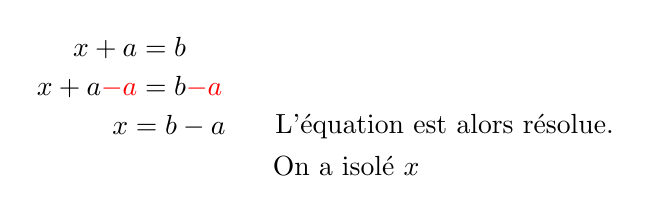
\begin{tikzpicture}
\node at (15, 3) {$ x+a=b$} ; 
\node at (15, 2.5) {$ x + a \textcolor {red} {-a} = b \textcolor {red}{-a}$} ; 
\node at (15.5, 2) {$ x = b-a $} ;  
\node at (19, 2) {L'équation est alors résolue.} ;  
\node at (17.75 , 1.5) {\vocabulaire{On a isolé $x$}} ;  
\end{tikzpicture}    
 
\bigskip 

\Asavoir{{\large 2) }\underline{Équations de la forme $ax=b$}} 

Pour isoler $x$, on multiplie par $\textcolor{red}{\dfrac{1}{a}}$  chaque membre 



\begin{tabular}{M{3.5cm}M{10cm}}
$ ax=b$   & \\
$   \textcolor {red} {\dfrac{1}{\cancel{a}}} \times \cancel{a}x = b \times \textcolor {red}{\dfrac{1}{a}}$   \\
$ x = b-a $   & 
L'équation est alors résolue.  \\
\vocabulaire{On a isolé $x$}  \\ 
\end{tabular}     
   
\bigskip 

\Asavoir{{\large 3) }\underline{Équations de la forme $ax + b = c$}} 

\medskip

Pour isoler $x$, on applique \ding{172}, puis \ding{173}.

\medskip

\newcommand{\xdownarrow}[1]{%
  {\left\downarrow\vbox to #1{}\right.\kern-\nulldelimiterspace}
}

\begin{tabular}{ll}
$ ax + b = c$   & \multirow{2}{5cm}{\methode{ $\Big\downarrow$ On applique \ding{172}} } \\
$  ax + b \textcolor {red} {-b} = c  \textcolor {red} {-b}  $  &   \\
$  ax = c -b $ & \methode{On se retrouve en \ding{173}} \\
$   \textcolor {red} {\dfrac{1}{\cancel{a}}} \times \cancel{a}x = (c - b) \times \textcolor {red} {\dfrac{1}{a}}$  & \methode{$\Big\downarrow$ On applique \ding{173}} \\
$ x = \dfrac{c-b}{a}$   & \multirow{2}{5cm} { L'équation est alors résolue. \\
 \vocabulaire{On a isolé $x$} } \\ 
\end{tabular} 

   
\bigskip 

\Asavoir{{\large 4) }\underline{Équations de la forme $ax + b = cx + d$}} 

\medskip

Pour isoler $x$, on ajoute $\textcolor{red}{-cx}$ à chaque membres et on est alors ramené au cas 
\ding{174}.

\medskip

\begin{tabular}{ll}
$ ax + b = cx +d $   & \multirow{2}{5cm}{\methode{ $\Big\downarrow$ On soustrait \textcolor{red}{cx} }} \\
$ \textcolor{red}{-cx} + ax + b = \textcolor{red}{-cx} + cx +d $   & \\
$  -cx +ax + b \textcolor {red} {-b} = d  \textcolor {red} {-b}  $  &   \\
$  (a - c)x   = d $ & \methode{On se retrouve en \ding{174}} \\
$  (a - c)x   = d  -b $ & \methode{$\big\downarrow$  On applique le cas  \ding{172}} \\
$  x = \dfrac{d-b}{a-c}$  & \methode{$\Big\downarrow$ On applique \ding{173}} \\
\end{tabular} 

 L'équation est alors résolue. \\   \vocabulaire{On a isolé $x$}  \\ 

   
\bigskip 

\Asavoir{{\large 5) }\underline{Équations d'autres formes}}


\medskip


En développant les calculs, et en simplifiant, on pourra toujours, en quatrième, se ramener au cas  \ding{172}, \ding{173}, \ding{174} ou \ding{175}.

\newpage

                 
                 \intitule{Équations du premier degré} 
                 
                 \centerline{\Asavoir{\Large Exemples rédigés de cinq types}}   
                 
\bigskip                  
                 
                 
\Asavoir{{\large 1) }\underline{Équations de la forme $x +a = b$}}   \hspace*{2cm} \vocabulaire{Cas 1}

\bigskip 

\begin{tabular}{lM{3cm}|M{1cm}l}

$x+3 = 0$ & \multirow{2}{3cm}{\methode{$\Big\downarrow$ On ajoute -3} }  & & $x +3 = 7 $\\
$x=-3$   &  & & $x+3 -3 = 7 -3 $\\
  &  & & $x = 4 $\\
$\mathcal{S} =\left\lbrace -3 \right\rbrace$ &  & & $\mathcal{S} =\left\lbrace 4 \right\rbrace$ \\  
  
\end{tabular}
              
\bigskip                  
                 
                 
\Asavoir{{\large 2) }\underline{Équations de la forme $ax = b$}}   \hspace*{2cm} \vocabulaire{Cas 2}

\bigskip 

\begin{tabular}{lM{3.5cm}|M{1cm}l}

$2x = 0$ & \multirow{2}{3cm}{\methode{$\Big\downarrow \mathrm{On\; multiplie\; par\; } \dfrac{1}{2}$} }  & & $2x = 3 $\\
$ \cancel{2}x \textcolor{red}{\times \dfrac{1}{\cancel{2}}}=0$   &  & & $ \cancel{2}x \textcolor{red}{\times \dfrac{1}{\cancel{2}}} = 3 \textcolor{red}{\times \dfrac{1}{2}} $\\
& & & $x = \dfrac{3}{2}$\\
$\mathcal{S} =\left\lbrace 0 \right\rbrace$ &  &  & $\mathcal{S} =\left\lbrace \dfrac{3}{2} \right\rbrace$ \\  
\end{tabular}

\bigskip                  
              
                 
\Asavoir{{\large 3) }\underline{Équations de la forme $ax +b = c$}} 

\bigskip 

\begin{tabular}{lM{4cm}|M{1cm}l}

$4x + 5 = 0$ & 
   \multirow{2}{3cm}{\vocabulaire {$\approx$  \ding{172}} \methode{$\Big\downarrow$ On ajoute -5} }  & & $9x + 6 = - 7 $\\
$4x= -5 $   &  & &$9x + 6 -6   = - 7 -6 $\\
$\cancel{4}x \times \dfrac{1}{\cancel{4}} = - 5 \times \dfrac{1}{4} $  & 
   \multirow{3}{4cm}{\vocabulaire {$\approx$  \ding{173}} \methode{$\Big\downarrow \mathrm{On\; multiplie\; par\; } \dfrac{1}{4}$}}  & & $9x = -13  $\\
 &  & & $ \dfrac{1}{\cancel{9}} \times \cancel{9}x = -13 \times \dfrac{1}{9} $\\   
$x = -\dfrac{5}{4} $   &  & & $x = - \dfrac{13}{9} $\\
 &  & & \\  
$\mathcal{S} =\left\lbrace -\dfrac{5}{4} \right\rbrace$ & \multicolumn{1}{c|}{\methode {Fini}} & &  $\mathcal{S} =\left\lbrace  -\dfrac{13}{9} \right\rbrace$ \\    
\end{tabular}          
  

\bigskip                  
 
             
                 
\Asavoir{{\large 4) }\underline{Équations de la forme $ax +b = cx +d $}} 

\bigskip 

\iffalse 


\makeatletter
\newdimen\multi@col@width
\newdimen\multi@col@margin
\newcount\multi@col@count
\multi@col@width=0pt
\tikzset{
  multicol/.code={%
    \global\multi@col@count=#1\relax
    \global\let\orig@pgfmatrixendcode=\pgfmatrixendcode
    \global\let\orig@pgfmatrixemptycode=\pgfmatrixemptycode
    \def\pgfmatrixendcode##1{\orig@pgfmatrixendcode%
      ##1%
      \pgfutil@tempdima=\pgf@picmaxx
      \global\multi@col@margin=\pgf@picminx
      \advance\pgfutil@tempdima by -\pgf@picminx
      \divide\pgfutil@tempdima by #1\relax
      \global\multi@col@width=\pgfutil@tempdima
      \pgf@picmaxx=.5\multi@col@width
      \pgf@picminx=-.5\multi@col@width
      \global\pgf@picmaxx=\pgf@picmaxx
      \global\pgf@picminx=\pgf@picminx
      \gdef\multi@adjust@position{%
        \setbox\pgf@matrix@cell=\hbox\bgroup
        \hfil\hskip-\multi@col@margin
        \hfil\hskip-.5\multi@col@width
        \box\pgf@matrix@cell
        \egroup
      }%
      \gdef\multi@temp{\aftergroup\multi@adjust@position}%
      \aftergroup\multi@temp
    }
    \gdef\pgfmatrixemptycode{%
      \orig@pgfmatrixemptycode
      \global\advance\multi@col@count by -1\relax
      \global\pgf@picmaxx=.5\multi@col@width
      \global\pgf@picminx=-.5\multi@col@width
      \ifnum\multi@col@count=1\relax
       \global\let\pgfmatrixemptycode=\orig@pgfmatrixemptycode
      \fi
    }
  }
}
\makeatother

\fi

\setbox1=\vtop{ \hsize=5cm \null % null assure l'alignement par le haut 
\begin{tikzpicture}% [every node/.style={anchor=west}]
  \matrix (m) [matrix of math nodes,
row sep=0cm,column sep=0cm,  
% nodes={rectangle, draw},  
%    nodes in empty cells,
column 1/.style={anchor=base east},
column 3/.style={anchor=base west}]{
3x -5                                         &=& x + 1  \\%  
3x \; \TextSoulign{blue}{-x} -5               &=& x +1 \;\TextSoulign{blue}{-x} \\
2x -5                                         &=& |(a)| 1  \vocabulaire{\hspace{1.5cm}\text{\ding{174}}} \\
2x -5 \; \TextSoulign{blue}{+5}               &=& |(b)|1+\;\TextSoulign{blue}{5}       \\
2x                                            &=& 6 \vocabulaire{\hspace{1.5cm}\text{\ding{173}}} \\
2x \; \TextSoulign{blue}{\times \dfrac{1}{2}} &=& 6 \;\TextSoulign{blue}{\times \dfrac{1}{2}}  \\
x                                             &=& 3 \\
 \hbox to .1cm{}                              & &   \\
\textcolor{white}{\mathcal{S} = \left\lbrace -\dfrac{5}{4} \right\rbrace}& & \hbox to .1cm{}\\
}; 
\draw[color=blue,->,>=latex] (a) to[out=0,in=0]node[midway,below]
{\vocabulaire {\ding{172}}}   (b);       
\node[fit=(m-9-1)(m-9-3)]{$\mathcal{S} = \left\lbrace 3 \right\rbrace$};      
\end{tikzpicture}}

\setbox2=\vtop { \hsize=5cm  \null
\begin{tikzpicture}% [every node/.style={anchor=west}]
  \matrix (n) [matrix of math nodes,
row sep=0cm,column sep=0cm,  
% nodes={rectangle, draw},  
%    nodes in empty cells,
column 1/.style={anchor=base east},
column 3/.style={anchor=base west}]{
|(c)|   3x -5    &=& |(d)|  9x +1 \\
 \hbox to .1cm{} & &   \\               
|(e)| 3x -9x     &=& |(f)| 1 + 5    \\
 -6x &=& |(g)| 6 \\   
x &=& |(h)| \dfrac{6}{-6} \\   
x &=& -1  \\
 \hbox to .1cm{}                              & &   \\
\textcolor{white}{\mathcal{S} = \left\lbrace -1 \right\rbrace}& & \hbox to .1cm{} & \\
 }; 
\draw[color=blue,->,>=latex] (c) to[out=-30,in=110]node[midway,right] {} (f) ;   
\draw[color=blue,->,>=latex] (d) to[out=190,in=north east]node[midway,right] {} (e) ;  
\draw[color=blue,->,>=latex] (g) to[out=0,in=0]node[midway,right] {\methode{On divise par -6}} (h) ;    
\node[fit=(n-8-1)(n-8-3)]{$\mathcal{S} = \left\lbrace -1 \right\rbrace$};         
\end{tikzpicture}}


\centerline{ \box1 \quad\vrule\quad \box2 \hfill}

\newpage

\Asavoir{{\large 5) }\underline{Plus dur ...}} 

\medskip 

\begin{tikzpicture}% [every node/.style={anchor=west}]
  \matrix (m) [matrix of math nodes,
row sep=0cm,column sep=0cm,  
% nodes={rectangle, draw},  
%    nodes in empty cells,
column 2/.style={anchor=base east},
column 4/.style={anchor=base west}
]{
\Asavoir{\large a) } & 6 \textcolor{blue}{\underbrace{\textcolor{black}{-4 (1-x)}}} &=& |(a)| 3x + 5 \\
   & 6  -4 \times 1 - 4\times (-x) &=& |(b)| 3x + 5  \\
   & 6  -4  + 4x &=&  3x + 5  \\   
   & 2  + 4x &=&  3x + 5  \\   
   & 2  + 4x -3x &=& 3x + 5 -3x  \\   
   & 2 + x      &=& 5 \\
   & 2  + x -2 &=& 5 -2 \\     
   & x &=& 3 \\  
 \hbox to .1cm{}                              & &   \\   
   & & & \hspace*{1cm}\mathcal{S} =\left\lbrace 3 \right\rbrace \\        
}; 
\node [right = 1cm of a.west] (c) {} ; 
\node [right = 1cm of b.west] (d) {} ; 
\draw[color=blue,->,>=latex] (c) to[out=0,in=0] node[midway,right] {\hspace*{.5cm} \parbox{3cm}{Ne ressemble pas à\\ un cas connu ...\\
On développe }}  (d) ; 
\end{tikzpicture}


\bigskip 

\begin{tikzpicture}% [every node/.style={anchor=west}]
  \matrix (m) [matrix of math nodes,
row sep=0cm,column sep=0cm,  
% nodes={rectangle, draw},  
%    nodes in empty cells,
column 2/.style={anchor=base east},
column 4/.style={anchor=base west}
]{
\Asavoir{\large b) } 
   & 3 - \big[5 -(x-7)\big] &=& |(a)| 2(x-4)-1 \\
   & 3 - (5 -x +7)          &=& |(b)| 2x-2\times 4 -1 \\
   &3 -5 +x -7              &=&  2x -8 -1 \\     
   & x - 9                  &=& |(c)| 2x - 9   \\   
   & x                      &=& |(d)| 2x \\     
   & x                      &=& |(i)| 0 \\  
 \hbox to .1cm{}                              & &   \\    
   & & & \hspace*{1.5cm}\mathcal{S} =\left\lbrace 0 \right\rbrace \\         
}; 
\node [right = 2cm of a.west] (e) {} ; 
\node [right = 1cm of b.west] (f) {} ; 
\draw[color=blue,->,>=latex] (e) to[out=0,in=0] node[midway,right]{\hspace*{.5cm} On développe ...} (b); \\ 
\node [right = 1.5cm of c.west] (g) {} ; 
\node [right = 1.25cm of d.west] (h) {} ; 
\draw[color=blue,->,>=latex] (g) to[out=0,in=0] node[midway,right]{\hspace*{.5cm} On soustrait 9} (h); \\ 
\node [right = 1cm of d.west] (k) {} ; 
\node [right = 1cm of i.west] (j) {} ; 
\draw[color=blue,->,>=latex] (k) to[out=0,in=0] node[midway,right]{\hspace*{.5cm} On soustrait $x$ à gauche et à droite} (j); \\ 
\end{tikzpicture} 

\newpage 


\ifdefined\COMPLETE
\else
    \end{document}
\fi